Den experimentella datainsamlingen bestod av två olika uppställningar för att tillsammans svara på de två respektive frågeställningarna. I del 1 undersöktes stötar i en dimension och deras stötkoefficient. I del 2 utvidgades undersökningen till två dimensioner och även fördelning av energi, rörelsemängd och rörelsemängdsmoment i två dimensioner undersöktes. Nedan redovisas det material, uppställningar och tillvägagångssätt som användes.

\subsection{Material och uppställning} 

För del 1 användes ryttare av metall på en luftskena för att modellera endimensionella stötar, enligt figur \ref{fig:del1}. Luftskenan var av modell Pasco physics airtrack (SF-9214) och var hopkopplad med en luftfläkt av modell Frederiksen Air Blower 1970,70. Ovanpå själva ryttarna som gled längs luftskenan placerades två metallvikter och reflextejp för att mäta ryttarnas position med ett kamerasystem. De extra vikterna placerades på toppen i syfte att förskjuta masscentrum uppåt och därmed minska impulsmomentet i stötarna och således motverka oönskad rörelse i $\hat z$-led. I den ena mätserien försågs även en av ryttarna med en anordning beståendes av en klyka med gummiband. Detta för att undersöka hur materialet i kollisionspunkten påverkar stötkoefficienten.

\begin{figure}[H]
    \centering
    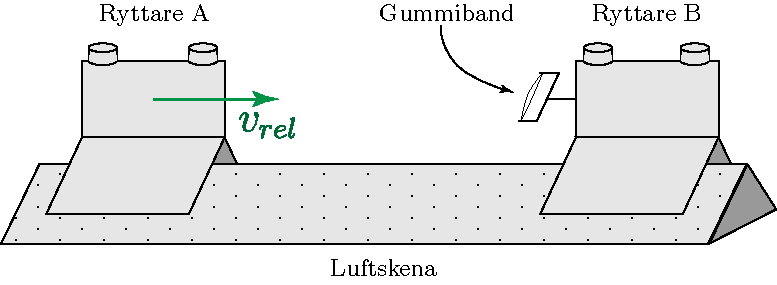
\includegraphics[width=0.8\linewidth]{images/metod/ryttare.pdf}
    \caption{Försöksuppställningen för endimensionella stötar. Två ryttare på en luftskena kolliderade med relativ hastighet $v_{\text{rel}}$. I första mätserien utgjordes deras kontaktpunkt av ett uppspänt gummiband. I den andra skedde kollisionen metall mot metall.}
    \label{fig:del1}
\end{figure}

 För del 2 användes istället ett luftbord med två metallpuckar, enligt figur \ref{fig:del2}, för att undersöka stötar i två dimensioner. Luftbordet kopplades i sin tur till samma luftfläkt som i del 1. Utanpå puck A placerades ett gummiband i syfte att öka friktionen mellan kontaktytorna vid stötarna. Ovanpå vardera puck placerades även tre bitar reflextejp för att mäta position och rotation. Bitarna placerades på randen för att möjliggöra numerisk beräkning av masscentrums translation och rotation med hög precision.
 
 Utöver utrustningen för respektive uppställningen användes även ett motion capture system från {Qualisys} av modell Oqus 300 monterat i taket för att mäta objektens position över tid med upplösning \(\SI{e-6}{m}\). Kamerasystemets uppdateringsfrekvsens valdes till 500 Hz för att erhålla högre upplösning i tid och med större noggrannhet bestämma kollisionsögonblicket.

\begin{figure}[H]
    \centering
    \begin{subfigure}{.5\textwidth}
        \centering
        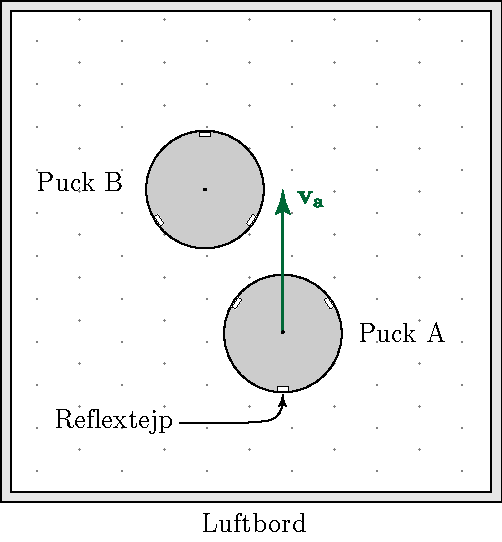
\includegraphics[width=0.95\linewidth]{images/metod/del2_bord.pdf}
        \caption{Uppställningen för de tvådimensionella stötarna av puckar på luftbord. Puck A kolliderade med initialhastighet $v_a$ i puck B. Längs puckarnas rander placerades reflextejp.}
        \label{fig:del2_bord}
    \end{subfigure} 
    \hfill
    \begin{subfigure}{.45\textwidth}
        \centering
        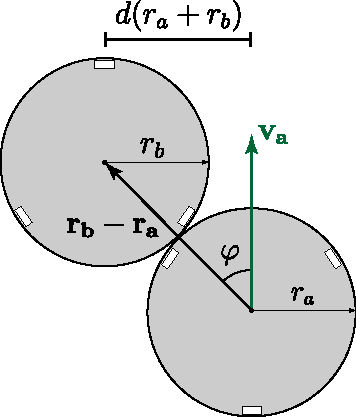
\includegraphics[width=0.75\linewidth]{images/metod/del2_kollision.pdf}
        \caption{Kollisionsparametrar för puckarna. Utskrivna är den icke-normaliserade kollisionspunkten $d(r_a+r_b)$, hastighetsvektorn $v_a$, ortsvektorn mellan masscentran $\mathbf{r_b}-\mathbf{r_a}$, relativa vinkeln $\varphi$ och radierna $r_a$ och $r_b$.}
        \label{fig:del2_collision}
    \end{subfigure}
    \caption{Försöksuppställning för de tvådimensionella stötarna på luftbordet sedd ovanifrån och deras kollisionsparametrar.}
    \label{fig:del2}
\end{figure}

\subsection{Genomförande} \label{chap:material}
Innan mätningarna genomfördes kalibrerades bordets och skenans lutning samt deras lufttillförsel för att minimera icke önskvärd energipåverkan i systemet. Konktaktytor torkades sedan av med desinfektionsdukar för att avlägsna ytbeläggningar av smuts och tejprester. Även kamerasystemet kalibrerades med tillhörande kalibreringsutrustning tills en residual runt $\SI{2e-4}{m}$ erhölls. I både del 1 och 2 mättes objektens relevanta konstanter innan med mätutrustning från labbsalen, se tabell \ref{tab:mätutr.}. I del 1 mättes massorna och i del 2 mättes massorna och radierna, se tabell \ref{tab:prop1} och \ref{tab:prop2}.

I första mätserien för del 1 monterades klykan med gummiband på ryttare B. Därefter placerades de på luftskenan och skickades iväg för hand mot varandra drygt 50 gånger med godtyckligt varierad relativ hastighet. För varje stöt startades en ny mätning med kamerasystemets mjukvara, Qualisys Tracking Manager (QTM), som löpande registrerade ryttarnas position. I den andra mätserien genomfördes samma procedur efter att klykan monterats av så att ryttarnas metallsidor blev ny kontaktpunkt.  %Ev. förklara lika hastigheter

Utifrån den erhållna positionsdatan beräknades den relativa kollisionshastigheten $v_{\text{rel}}$ innan kollisionsögonlicket samt stötkoefficienten $e$ med datanalys i \textit{Python}, se listing \ref{lst:1main} i bilaga \ref{bil:kod}. Koefficienten beräknades genom att ta medelvärdet av $v_{\text{rel}}$ under 0,2 sekunder innan och efter stöten för att sedan dividera dem enligt ekvation \eqref{ekv:e}. %Ev förklara varför 0.2s

I del 2 placerades puckarna på luftbordet där puck A sköts för hand mot den stillastående pucken B. Detta skedde drygt 50 gånger där vinkel och träffpunkt varierades godtyckligt. Utifrån den insamlade positionsdatan från markörerna på randen beräknades initialt puckarnas masscentrums translation och rotation numeriskt, se bilaga \ref{bil:kod} tabell \ref{lst:2center_calc}. Utifrån det beräknades därefter puckarnas translationshastighet $\mathbf{v_i}$, vinkelhastighet $\omega_i$, rörelsemängd $\mathbf{p_i}$, rörelsemängdsmoment $\mathbf{L_{MC}}_i$ och kinetiska energi $T_i$ numeriskt enligt dataanalysen i bilaga \ref{bil:kod} och teorin i avsnitt \ref{sec:teori}. För att besvara frågeställningen om bevaring och fördelning innan och efter stöt studerades enbart medelvärdet av parametrarna 0,2 sekunder innan och efter kollisionstillfälle. Kollisionspunkten $d$ definierades däremot som det normerade avståndet mellan masscentran vinkelrät mot hastighetsvektorn i kollisionsögonblicket. Kvoten beräknades enligt 
\begin{equation} \label{ekv:d_calc}
    d=\frac{\sin(\varphi)||\mathbf{r_b}-\mathbf{r_a}||}{(r_a+r_b)}.
\end{equation} %Gör tydligare skillnad på orts och radier
utifrån parametrarna redovisade i figur \ref{fig:del2_collision}.

Innan varje mätserie påbörjades genomfördes även en referensmätning av påverkan från eventuell friktion och luftströmmar. Objekten sköts över kollisionsområdet på luftskenan respektive luftbordet för att sedan numeriskt beräkna påverkan. 